\subsection*{Opdeling af tallyChars()}
en analyse af tallyChars() viser at der er 4 dele der kan undersøge:
\begin{itemize}
\item Reader
\item While loop
\item Try / catch
\item Map
\end{itemize}

\section*{Første forsøg}
Første forsøg var at kigge på try catch, da denne kan give et unødvendigt overhead.
En ikke så pæn løsning ser således ud:




\lstset{ %
language=Java,                % choose the language of the code
basicstyle=\footnotesize,       % the size of the fonts that are used for the code
numbers=left,                   % where to put the line-numbers
numberstyle=\footnotesize,      % the size of the fonts that are used for the line-numbers
stepnumber=1,                   % the step between two line-numbers. If it is 1 each line will be numbered
numbersep=5pt,                  % how far the line-numbers are from the code
backgroundcolor=\color{white},  % choose the background color. You must add \usepackage{color}
showspaces=false,               % show spaces adding particular underscores
showstringspaces=false,         % underline spaces within strings
showtabs=false,                 % show tabs within strings adding particular underscores
frame=single,           % adds a frame around the code
tabsize=2,          % sets default tabsize to 2 spaces
captionpos=b,           % sets the caption-position to bottom
breaklines=true,        % sets automatic line breaking
breakatwhitespace=false,    % sets if automatic breaks should only happen at whitespace
escapeinside={\%*}{*)}          % if you want to add a comment within your code
}



\begin{lstlisting}
        int b; // will be slower, only check for lowercase chars
        boolean check[] = new boolean[60];
        while ((b = reader.read()) != -1) { // Big O = N
            if((b>96 && b<123)) {
             int c=b-97; // a = 0
                if(check[c]) {
                    freq.put(b, freq.get(b) + 1);
                }
                else {
                    freq.put(b, 1L);
                    check[c]= true;
                }
            }
        }
\end{lstlisting}


\newpage
\begin{figure}
  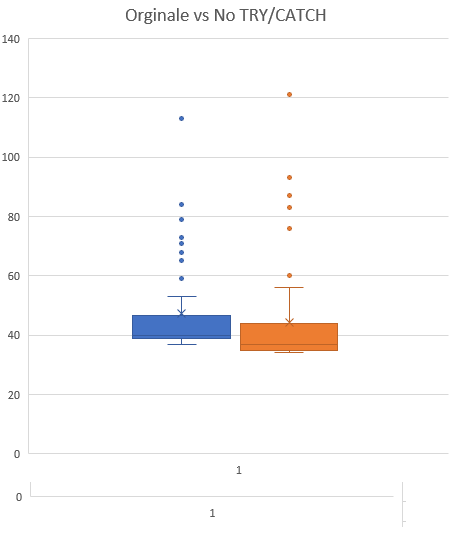
\includegraphics[width=0.4\linewidth]{orginalboksvstry.png}
  \caption{Boksplot af det orginale program mod en no Try/catch}
  \label{fig:orginalvstry}
\end{figure}
Ved hurtigt øjekast ser no try/catch lidt hurtigere ud, men i løsninger bliver kun små bogstaver talt, og at lave et program der også tager de store, vil kun lægge tid til, og ikke blive hurtigere. Så denne løsningen der ikke arbejdet videre med.
\newpage


\section*{Andet forsøg}
Dette forsøg er der kigget på Map funktionen, for at lave en bedre Map funktion er følgende kode lagt prøvet:

\begin{lstlisting}
int b;
	while ((b = reader.read()) != -1) {
		freq.merge(b,1L,Long::sum);
        }
\end{lstlisting}
Dette gør at der ikke er brug for en Try/catch, eller en speciel måde at håndtere om et map er tomt eller ej.

\newpage
\begin{figure}
  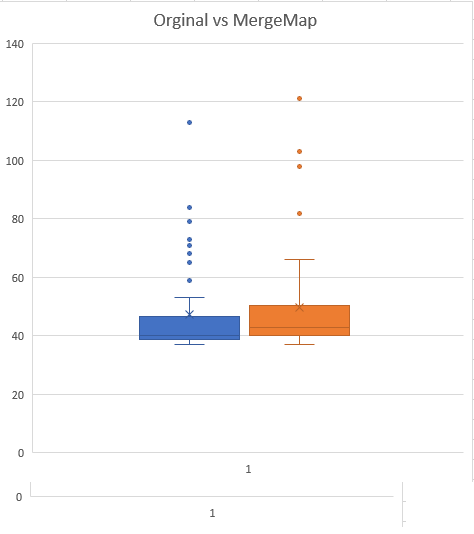
\includegraphics[width=0.4\linewidth]{orginalboksvsmerge.png}
  \caption{Boksplot af det orginale program mod en MergeMap}
  \label{fig:orginalvsmerge}
\end{figure}
denne løsning, selve om den ser langt pænere ud, tog faktisk længere tid at udføre end det orginale program. Derfor er denne linie af forsøg stoppet.
\newpage

\subsection*{Tredje forsøg}
Dette ville have dækket over en while loop, men dette forsøg er udskudt, da det ikke virker fornuftigt at problemet skulle være her.



\subsection{Fjerde forsøg}
Sidste forsøg er på Reader, her er der forsøgt at udskift en BufferedReader, således at der ikke hvergang skal hentes et tegn fra filen, men derimod fra en buffer.

Koden er som følger:
\begin{lstlisting}
    private static void tallyChars(BufferedReader reader, Map<Integer, Long> freq) throws IOException {
        int b;
        while ((b = reader.read()) != -1) {
            freq.merge(b,1L,Long::sum);
        }
    }
\end{lstlisting}

\newpage
\begin{figure}
  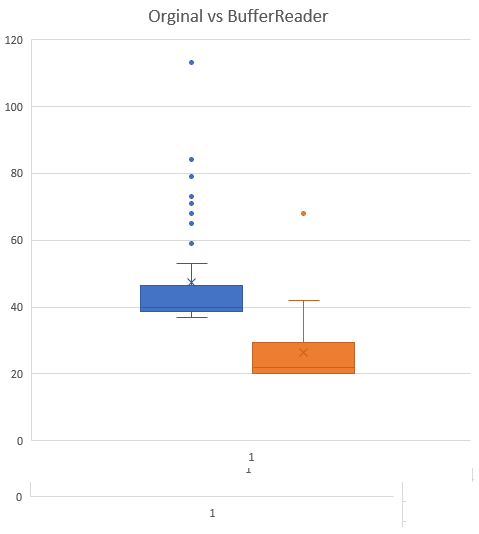
\includegraphics[width=0.4\linewidth]{orginalboksvsbuffer.png}
  \caption{Boksplot af det orginale program mod en BufferReader}
  \label{fig:orginalvsbuffer}
\end{figure}
Denne løsning, bliver det hele markant hurtigere som kan ses af boksplotten.
Forskelle skyldes at programmet ikke skal tilgå filen for hver karakter, men derimod load det ind i en buffer.
\newpage

Kigger vi på mean og standard deviation kan vi ses en næsten 100 procent forbedring af koden.

\begin{lstlisting}
mean is : 26,13 ms +/-  27,51 ms
mean is : 23,85 ms +/-  24,78 ms
mean is : 23,48 ms +/-  24,40 ms
mean is : 22,99 ms +/-  23,75 ms
mean is : 22,69 ms +/-  23,32 ms
mean is : 22,44 ms +/-  22,99 ms
mean is : 22,39 ms +/-  22,89 ms
mean is : 22,20 ms +/-  22,65 ms
mean is : 22,13 ms +/-  22,54 ms
mean is : 22,04 ms +/-  22,42 ms
mean is : 21,98 ms +/-  22,34 ms
mean is : 21,98 ms +/-  22,33 ms
mean is : 21,90 ms +/-  22,23 ms
mean is : 21,84 ms +/-  22,15 ms
mean is : 21,80 ms +/-  22,09 ms
mean is : 21,74 ms +/-  22,02 ms
mean is : 21,70 ms +/-  21,97 ms
mean is : 21,67 ms +/-  21,91 ms
mean is : 21,63 ms +/-  21,87 ms
mean is : 21,62 ms +/-  21,86 ms
mean is : 21,62 ms +/-  21,86 ms
mean is : 21,61 ms +/-  21,84 ms
mean is : 21,62 ms +/-  21,85 ms
mean is : 21,63 ms +/-  21,86 ms
mean is : 21,63 ms +/-  21,85 ms
mean is : 21,78 ms +/-  22,26 ms
mean is : 21,75 ms +/-  22,21 ms
mean is : 21,72 ms +/-  22,17 ms
mean is : 21,70 ms +/-  22,14 ms
mean is : 21,68 ms +/-  22,10 ms
mean is : 21,65 ms +/-  22,06 ms
mean is : 21,63 ms +/-  22,02 ms
mean is : 21,61 ms +/-  22,00 ms
mean is : 21,59 ms +/-  21,96 ms
mean is : 21,57 ms +/-  21,94 ms
mean is : 21,55 ms +/-  21,91 ms
mean is : 21,54 ms +/-  21,89 ms
mean is : 21,53 ms +/-  21,86 ms
mean is : 21,54 ms +/-  21,88 ms
mean is : 21,52 ms +/-  21,86 ms
mean is : 21,53 ms +/-  21,86 ms
mean is : 21,53 ms +/-  21,86 ms
mean is : 21,51 ms +/-  21,84 ms
mean is : 21,51 ms +/-  21,83 ms
mean is : 21,50 ms +/-  21,81 ms
mean is : 21,49 ms +/-  21,79 ms
mean is : 21,47 ms +/-  21,77 ms
mean is : 21,46 ms +/-  21,76 ms
mean is : 21,45 ms +/-  21,74 ms
mean is : 21,44 ms +/-  21,73 ms
\end{lstlisting}



